\chapter{Flutter Foundations}
\label{ch:flutter}
In the introduction, a new, promising, cross-platform framework was introduced. The Flutter's primary goal is to provide the ability to build high-performance, high-fidelity apps for \textit{iOS}, \textit{Android}, web, and desktop from a single code-base~\cite{flutter-technical-overview}. In this chapter, the framework's philosophy will be described. Used programming language and theory of reactive programming is briefly introduced. The chapter describes the concept of widgets as a base building block for every application. Later on, one of the most critical topic -- state management is discussed, its existing approaches and which to prefer when building applications. At the end of this chapter, the brief look under the framework's hood is discussed.

Flutter includes a modern react-style framework, a 2D rendering engine, predefined widgets and development tools. The primary premise is a motto "everything is a widget". A widget is an immutable building block of application which is part of the user interface. Each widget can define structural elements such as button, stylistic elements such as colour or it can define the interface's layout, such as padding. Widgets are composed as a tree hierarchy with composing each widget to another. If any event occurs (such as user interaction), the framework can rebuild part of this tree to redraw the screen.  

\begin{figure}[htp]
    \centering
    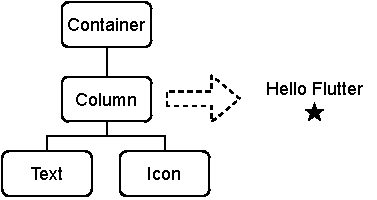
\includegraphics[width=0.5\linewidth]{img/flutter/hello-flutter.pdf}
    \caption{Widget composition example}
    \label{fig:hello-flutter}
\end{figure}

Flutter encourages developers to create and use small, single-purpose widgets and compose them to create complex interfaces and layouts. Take an~example from~\cref{listing:hello-flutter} , where, the root widget, Container is used to create a rectangular visual element. The Container is something like <div> element in HTML.  Under the Container is Column widget which composes children widgets into the vertical direction. Finally, Text widget displaying text "Hello Flutter" and Icon widget showing star icon. The~composition hierarchy along with a~result is shown at~\cref{fig:hello-flutter}.

\begin{listing}[ht]
\begin{minted}{dart}
Container(
    padding: const EdgeInsets.all(5.0),
    child: Column(
      mainAxisAlignment: MainAxisAlignment.center,
      children: [
        Text('Hello Flutter'),
        Icon(Icons.star),
      ],
    ),
),
\end{minted}
\caption{Widget composition code example}
\label{listing:hello-flutter}
\end{listing}
% ----- % ----- % ----- % ----- % ----- % ----- % ----- % ----- % ----- % ----- % ----- % ----- % ----- % ----- %
\section{Technical overview}
Flutter uses programming language Dart (specification v2.0~\cite{dart-specs}) also made by Google and is inspired by languages such as JavaScript. Dart using statically typed system with runtime checks, but like many other languages highly use type inference~\cite{dart-type-system}. Dart can be used from writing simple scripts to full-featured applications. The Dart has flexible compiler technology which can decide running code in different ways, depending on the targeted platform~\cite{dart-platforms}. 

\begin{itemize}
    \item \textbf{Dart Native} -- For programs targeting devices (mobile, desktop, server, and more), Dart Native includes both a Dart VM with \gls{jit} compilation and an~\gls{aot} compiler for producing machine code.
    \item \textbf{Dart Web} -- For programs targeting the web, Dart Web includes both a development time compiler (dartdevc) and a production time compiler (dart2js).
\end{itemize}

\begin{figure}[htp]
    \centering
    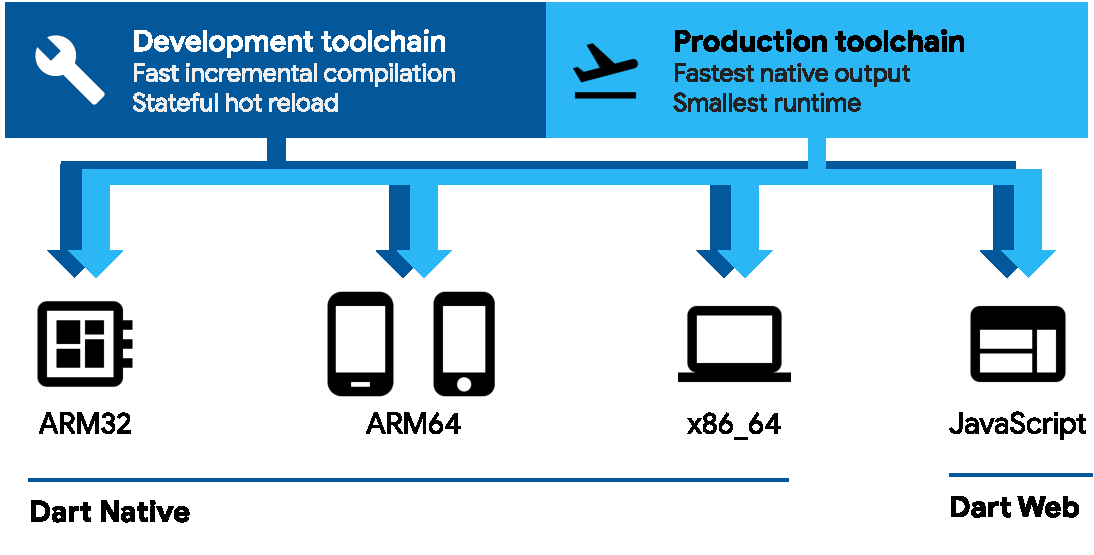
\includegraphics[width=0.8\linewidth]{img/flutter/dart-platforms.pdf}
    \caption{Dart platforms~\cite{dart-platforms}}
    \label{fig:dart-platform}
\end{figure}

Flutter performs the use of both ways. If the targeted platform is web, the \textit{Dart~Web} is used. For other platforms \textit{Dart~Native} is chosen. The Dart~Native's \gls{jit} compilation is highly used to support fast development process with ``hot-reload'' functionality. Then the~\gls{aot} compilation is used for the best-optimised production-ready result on the native platform.  

The Flutter framework is organised into several layers (see~\cref{fig:flutter-layer-cake}), where each layer makes usage of the previous one. The upper layers are more frequently used by developers on a daily basis, and lower layers are used only if the developers need to create particular customisations. 

\begin{figure}[htp]
    \centering
    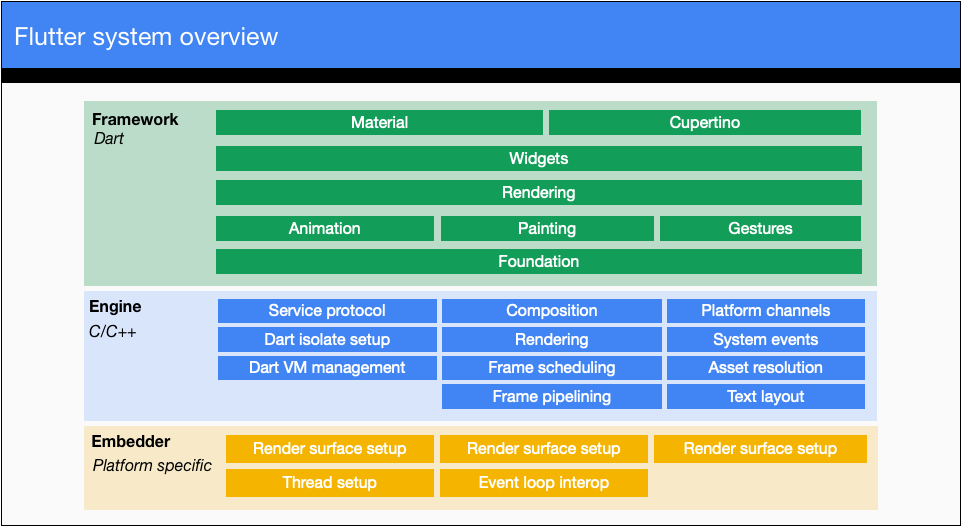
\includegraphics[width=0.8\linewidth]{img/flutter/flutter-layer-cake.png}
    \caption{Flutter system overview~\cite{flutter-technical-overview}}
    \label{fig:flutter-layer-cake}
\end{figure}

The Widgets layer defines all widget primitives such as Transform, Padding, Container and more. On top of that are \textit{Material} and \textit{Cupertino} layers which make use of the widgets from Widgets layer. These two layers offer developers set of predefined and highly customisable widgets which copies targeting platforms - \textit{Material} for \textit{Material Design} (Android systems) and \textit{Cupertino} for \textit{Apple Design} (iOS, macOS).  The~important thing is that with Flutter, these two top layers are not necessary to use, and developers can create their custom user interfaces whatever they like. 

% --- # --- # --- # --- # --- # --- # --- # --- # --- # --- # --- # --- # --- # --- # --- # --- # --- # --- #
\subsection{Reactive Programming}
The Flutter makes significant usage from the concept of reactive programming. With any application, there is a requirement to update data in response to user interaction or any other event such as getting data from the server. More than that, sometimes it is necessary to update different parts of the user interface in response to these events. 

The Flutter creates user interface by composing \textbf{immutable} widgets. The immutability is the key point here. Whenever user interface needs to "redraw" screen, the part of the widget tree is replaced by \textbf{new} widget instances (in fact, it is not simple as that, and this topic is more deeply discussed later in this chapter \todo{remove if not}).  In many other \gls{ui} frameworks, for example, in~\textit{Xamarin}, is usually taken the approach of coupling \gls{ui} components with so-called view-models through concepts such as data binding \todo{link to data binidng concept}. That means that whenever \gls{ui} needs to~change, the components mutate their states. Flutter takes an~entirely different approach. It can be said ``here is the current state of the application, draw something on the screen accordingly''.

\subsubsection{The Notion of Streams}
A Stream can be described as ``a pipe with two ends, only one allowing to insert something into it. When something is inserted into the pipe, it flows inside the pipe and goes out by the other end''~\cite{reactive-didier}. The Stream can convey any~data type, from simple values to~events, complex object or even another stream. The data can come to the Stream form example from an external data source such as server connection or from events such as user interactions. In Dart the Streams support manipulating them, filtering, re-grouping, modify data through the process and much more. This functionality can heavily be used to build reactive \gls{ui}. The~Flutter has several widgets supporting streams to rebuild part of the~\gls{ui} whenever new data arrived into the Stream.

The answer to the question ``what is reactive programming`` could be ``Reactive programming is programming with asynchronous data streams``~\cite{reactive-didier},\cite{reactive-red-hat}. Within Flutter framework, anything from an interaction event (tap, gesture), changes on a variable, messages, everything that may change is conveyed and triggered by streams.

That means that with reactive programming, according to~\cite{reactive-didier} the application 

\begin{quote}
    \begin{itemize}
        \item becomes asynchronous
        \item is architectured around the notion of Streams and their listeners
        \item when something happens somewhere (an event, a change of a variable …) a notification is sent to a Stream
        \item if ``somebody'' listens to that Stream, it will be notified and will take appropriate action(s), whatever its location in the application
    \end{itemize}
    
    From Widgets perspective -- Widget does not longer need to know
    
    \begin{itemize}
        \item what is going to happen next,
        \item who might use this information (no one, one or several Widgets)
        \item where this information might be used (nowhere, same screen, another one, several ones)
        \item when this information might be used (almost directly, after several seconds, never)
    \end{itemize}
\end{quote}

Later on in this chapter, the pattern Bussiness Logic Component (BLoC) is introduced. This pattern uses Streams to manage application life-cycle and state management. 
% ----- % ----- % ----- % ----- % ----- % ----- % ----- % ----- % ----- % ----- % ----- % ----- % ----- % ----- %
\section{Everything Is a Widget}
\todo{What is widget?}
\todo{widgets are not only visible UI}
\todo{stateles vs stateful widgets}
\todo{How Flutter rebuilds UI -- basic info about Widget Tree, Element Tree, State object, state comparison, const optimization}
\todo{starter counter example with setState()}

\todo{animations? -- good example of rebuilding part of UI}

% ----- % ----- % ----- % ----- % ----- % ----- % ----- % ----- % ----- % ----- % ----- % ----- % ----- % ----- %
\section{State Management}
\todo{Explain what is state management. Many approaches Provider, Staterebuilder, BLoC }

% ----- % ----- % ----- % ----- % ----- % ----- % ----- % ----- % ----- % ----- % ----- % ----- % ----- % ----- %
\section{Native Features}
\todo{How flutter can use native functions, e.g camera. Flutter plugins.}
% ----- % ----- % ----- % ----- % ----- % ----- % ----- % ----- % ----- % ----- % ----- % ----- % ----- % ----- %
\section{Flutter Internals}
\todo{Flutter canvas engine. Skia framework. How flutter internally works. Widget and widget tree concept. Tree shaking.}
\todo{Usage of Keys to prevent rebuilds}


